\documentclass[aspectratio=169]{beamer}

\usepackage{amsmath}
\usepackage{amssymb}
\usepackage{array}
\usepackage{xcolor}

\newcommand{\com}{\mathsf{Com}}

\definecolor{monerodark}{HTML}{4D4D4D}
\definecolor{monerorange}{HTML}{F26822}
\definecolor{text}{RGB}{248, 248, 242}

\setbeamercolor{normal text}{fg=text, bg=monerodark}
\setbeamercolor{title}{fg=text, bg=monerorange!90}
\setbeamercolor*{titlelike}{use=normal text}
\setbeamercolor*{frametitle}{use=normal text, bg=monerodark!80}
\setbeamercolor*{item}{fg=monerorange}

\setbeamertemplate{footline}[frame number]
\beamertemplatenavigationsymbolsempty

\title{Aura}
\subtitle{Using Privacy-Respecting Technology to Build Secure Voting}
\author{Aaron Feickert, Ph.D.}
\date{Monero Konferenco \\ 9 June 2024}

\begin{document}

\frame{\titlepage}

\begin{frame}{Acknowledgments and disclaimer}
	Aura is joint work with \textbf{Aram Jivanyan} of Firo and Yerevan State University. \\~\\

	The author is head of research at \textbf{Cypher Stack}, and research for Aura was conducted for \textbf{Firo}. \\~\\

	The material in this presentation is for informational use only, has not undergone formal external review, and does not constitute professional advice of any kind.
\end{frame}

\begin{frame}
    \begin{center}
        \Huge VOTING IS REALLY HARD
    \end{center}
    \vspace{30px}
    \begin{center}
        
\includegraphics[width=50px]{images/skull.png}
    \end{center}
\end{frame}

\begin{frame}
    \begin{center}
        \Huge DIGITAL VOTING IS EVEN HARDER
    \end{center}
    \vspace{30px}
    \begin{center}
        
\includegraphics[width=50px]{images/skull.png}
        
\includegraphics[width=50px]{images/skull.png}
    \end{center}
\end{frame}

\begin{frame}{What should it provide?}
    \begin{table}
        \centering
        \begin{tabular}{>{\arraybackslash}m{40px} >{\arraybackslash}m{100px} >{\arraybackslash}m{220px}}
            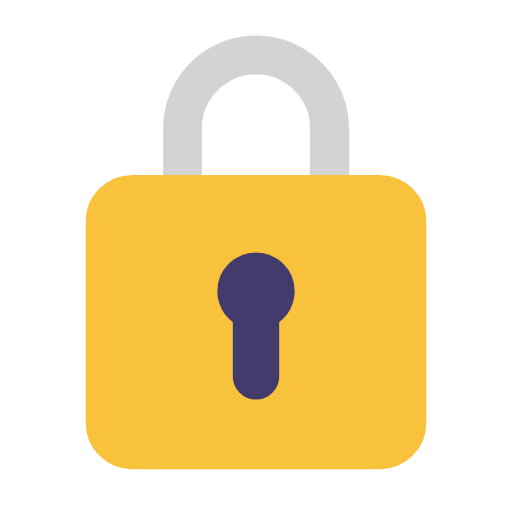
\includegraphics[width=30px]{images/lock.png} & \textbf{Ballot privacy} & Nobody can see ballot selections. \\
            
\includegraphics[width=30px]{images/detective.png} & \textbf{Voter privacy} & Nobody can see who cast a ballot. \\
            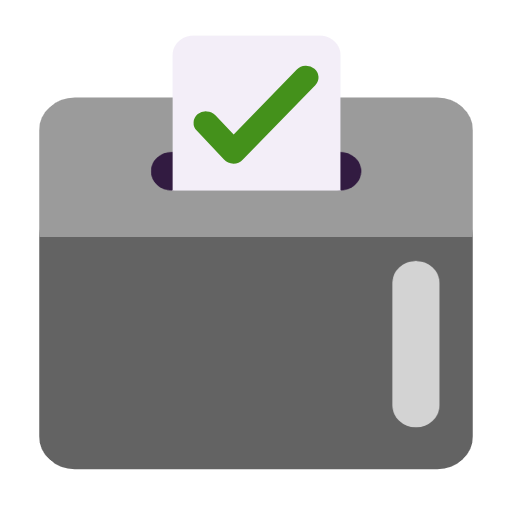
\includegraphics[width=30px]{images/ballot.png} & \textbf{Verifiability} & Everyone can prove the results are valid. \\
            
\includegraphics[width=30px]{images/evil.png} & \textbf{Trust minimization} & Evil officials shouldn't be able to cause damage. \\
        \end{tabular}
    \end{table}
\end{frame}

\begin{frame}{A case for ledgers}
    Distributed public ledgers are a great medium for this: they can be resistant to tampering and offer high availability. \\~\\

    The idea:
    \begin{table}
        \centering
        \begin{tabular}{>{\arraybackslash}m{40px} >{\arraybackslash}m{320px}}
            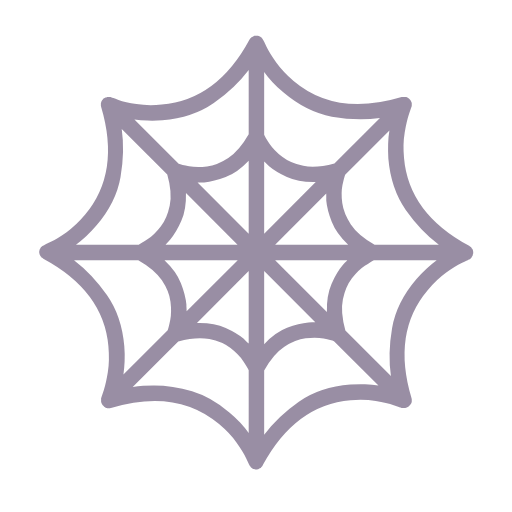
\includegraphics[width=30px]{images/web.png} & A voter submits a digital ballot to the network. \\
            
\includegraphics[width=30px]{images/ledger.png} & If valid, the ballot is added to the public ledger. \\
            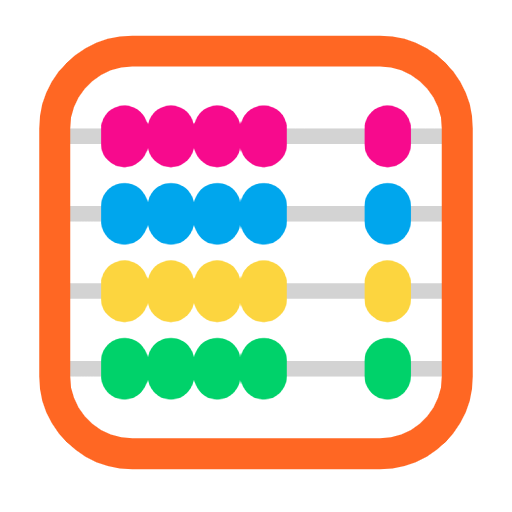
\includegraphics[width=30px]{images/abacus.png} & At the end of the election, ballots are tallied. \\
        \end{tabular}
    \end{table}

    But how can this meet our goals?
\end{frame}

\begin{frame}{Techniques from asset protocols}
    \begin{table}
        \centering
        \begin{tabular}{>{\arraybackslash}m{130px} >{\arraybackslash}m{40px} >{\arraybackslash}m{130px}}
            \textbf{Asset protocol} & & \textbf{Voting protocol} \\
            \hline
            Transactions are signed & 
\includegraphics[width=30px]{images/sign.png} & Ballots are signed \\
            Signatures are ambiguous & 
\includegraphics[width=30px]{images/question.png} & Signatures are ambiguous \\
            Amounts are encrypted & 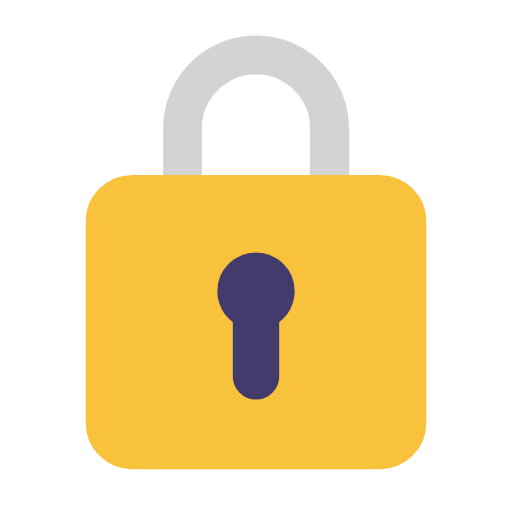
\includegraphics[width=30px]{images/lock.png} & Selections are encrypted \\
            Transactions are verifiable & 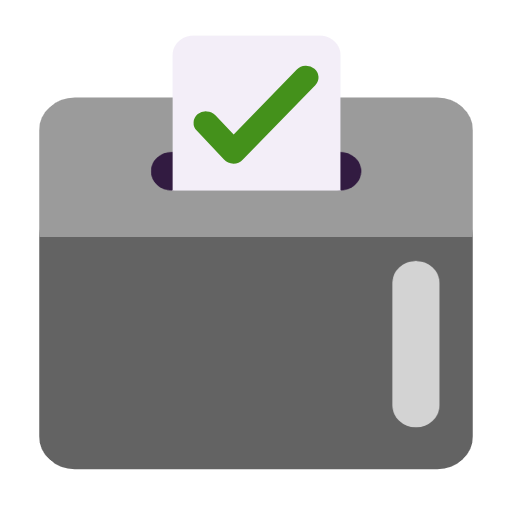
\includegraphics[width=30px]{images/ballot.png} & Ballots are verifiable \\
            Double spends are rejected & 
\includegraphics[width=30px]{images/x.png} & Double votes are rejected \\
        \end{tabular}
    \end{table}
\end{frame}

\begin{frame}{Aura}
    \textbf{Aura} is a design for privacy-respecting digital voting that does these things. \\~\\

    The players:
    \begin{table}
        \centering
        \begin{tabular}{>{\arraybackslash}m{40px} >{\arraybackslash}m{60px} >{\arraybackslash}m{220px}}
            
\includegraphics[width=30px]{images/crown.png} & \textbf{Organizer} & Sets up the election, talliers, and voters. \\
            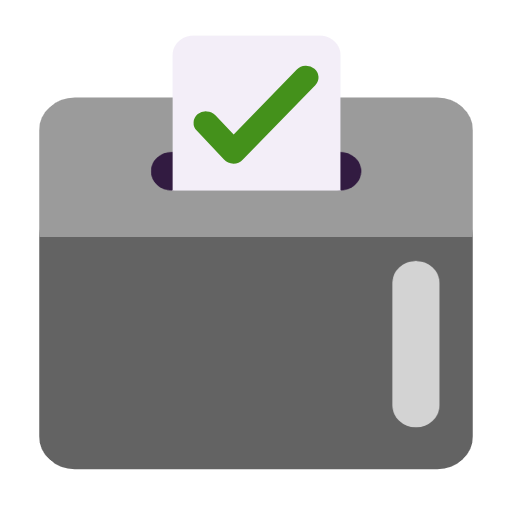
\includegraphics[width=30px]{images/ballot.png} & \textbf{Voter} & Casts a ballot. \\
            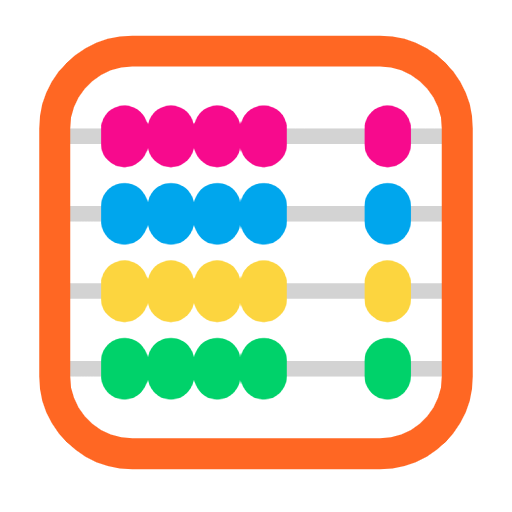
\includegraphics[width=30px]{images/abacus.png} & \textbf{Tallier} & Counts ballots to obtain the election results. \\
            
\includegraphics[width=30px]{images/check.png} & \textbf{Verifier} & Checks that the election results are valid. \\
        \end{tabular}
    \end{table}
\end{frame}

\begin{frame}{Ballot privacy}
    \begin{tabular}{>{\arraybackslash}m{40px} >{\arraybackslash}m{320px}}
        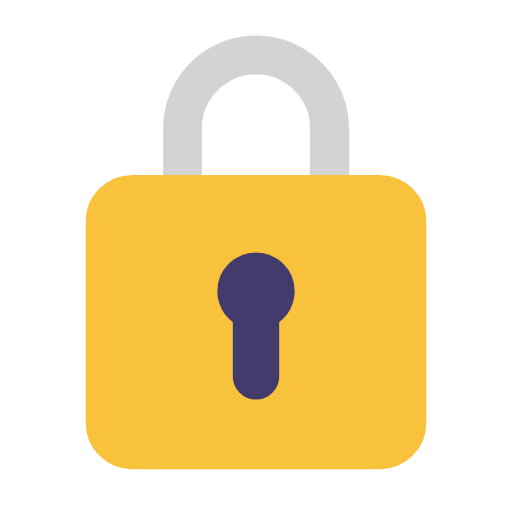
\includegraphics[width=30px]{images/lock.png} & We need to ensure that nobody can see the selections for a ballot. \\~\\
    \end{tabular}

    The voter uses (ElGamal) encryption to encrypt the selection for each option in its ballot so only the talliers can decrypt. \\~\\

    \begin{center}
        \begin{tabular}{>{\arraybackslash}m{15px} >{\arraybackslash}m{60px} >{\arraybackslash}{m}{40px} >{\arraybackslash}m{15px} >{\arraybackslash}m{60px}}
            
\includegraphics[width=15px]{images/x.png} & Alice & $\longrightarrow$ & 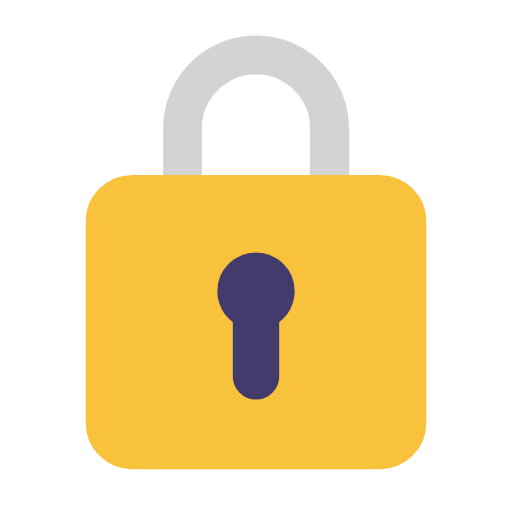
\includegraphics[width=15px]{images/lock.png} & Alice \\
            
\includegraphics[width=15px]{images/check.png} & Bob & $\longrightarrow$ & 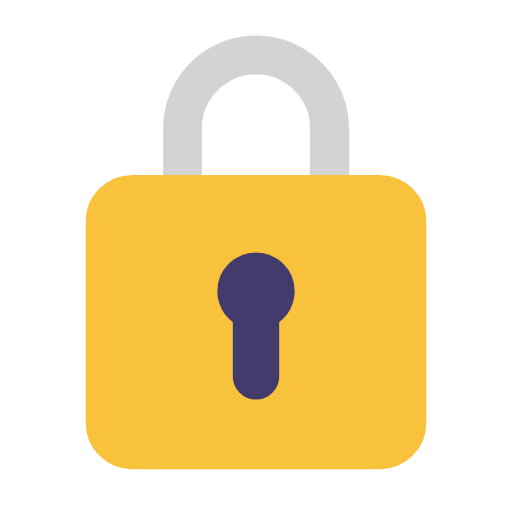
\includegraphics[width=15px]{images/lock.png} & Bob \\
            
\includegraphics[width=15px]{images/x.png} & Charlie & $\longrightarrow$ & 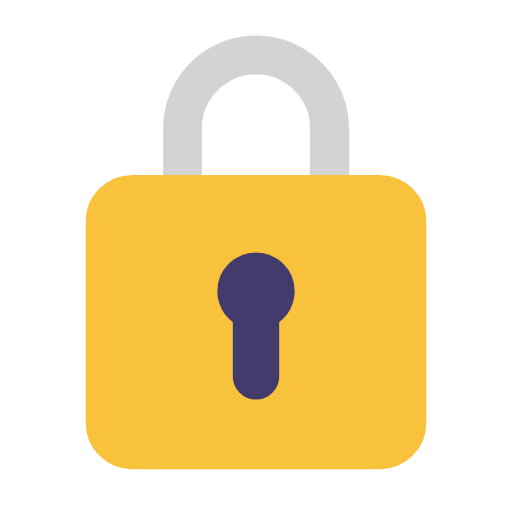
\includegraphics[width=15px]{images/lock.png} & Charlie \\
            
\includegraphics[width=15px]{images/x.png} & Dana & $\longrightarrow$ & 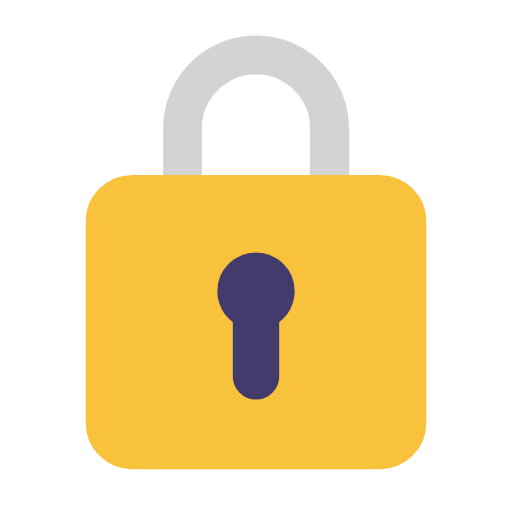
\includegraphics[width=15px]{images/lock.png} & Dana \\
            
\includegraphics[width=15px]{images/x.png} & Eve & $\longrightarrow$ & 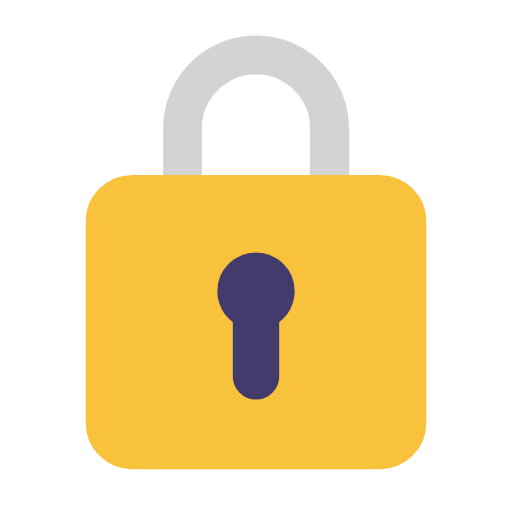
\includegraphics[width=15px]{images/lock.png} & Eve \\
        \end{tabular}
    \end{center}
\end{frame}

\begin{frame}{Verifiability}
    \begin{tabular}{>{\arraybackslash}m{40px} >{\arraybackslash}m{320px}}
        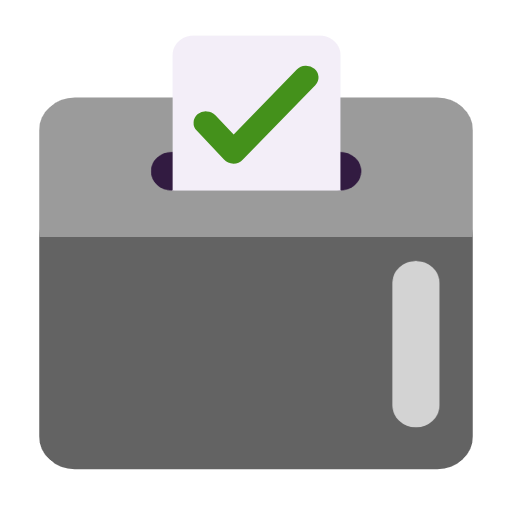
\includegraphics[width=30px]{images/ballot.png} & How do we know the voter didn't select more options than allowed, and encrypted the ballot properly? \\~\\
    \end{tabular}

    The voter includes zero-knowledge proofs:
    \begin{itemize}
        \item The ballot contains the allowed number of selections.
        \item The ballot is properly encrypted to the talliers. \\~\\
    \end{itemize}

    \begin{tabular}{>{\arraybackslash}m{40px} >{\arraybackslash}m{320px}}
        
\includegraphics[width=30px]{images/check.png} & An invalid ballot can be rejected from the ledger, and any verifier can check the proofs after the election. \\
    \end{tabular}
\end{frame}

\begin{frame}{Voter privacy}
    \begin{tabular}{>{\arraybackslash}m{40px} >{\arraybackslash}m{320px}}
        
\includegraphics[width=30px]{images/detective.png} & We need to ensure that nobody can see who cast a ballot. \\~\\
    \end{tabular}

    Each ballot is signed using something sort of like a linkable ring signature.
    It shows:
    \begin{itemize}
        \item The signer is on the list of allowed voters.
        \item The signer authorizes the ballot to be cast.
        \item The ballot has not been manipulated.
        \item The voter hasn't cast a ballot before. \\~\\
    \end{itemize}

    Crucially, it is not possible to determine which voter signed the ballot. \\~\\

    \begin{tabular}{>{\arraybackslash}m{40px} >{\arraybackslash}m{320px}}
        
\includegraphics[width=30px]{images/check.png} & An invalid ballot can be rejected from the ledger, and any verifier can check the signature after the election. \\
    \end{tabular}
\end{frame}

\begin{frame}{Tallying}
    \begin{tabular}{>{\arraybackslash}m{40px} >{\arraybackslash}m{320px}}
        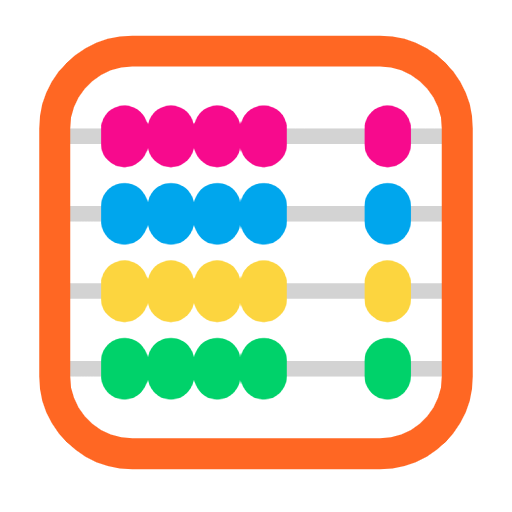
\includegraphics[width=30px]{images/abacus.png} & After the election, the talliers must count the ballots to obtain the results. \\~\\
    \end{tabular}

    Because they must not see the selections for any ballot, the talliers do the following:
    \begin{itemize}
        \item ``Add up'' the encrypted ballots.
        \item Collaboratively decrypt the summed ballots.
        \item Publish the total votes for each option. \\~\\
    \end{itemize}

    \begin{tabular}{>{\arraybackslash}m{40px} >{\arraybackslash}m{320px}}
        
\includegraphics[width=30px]{images/key.png} & Collaborative decryption is used since each tallier has only a portion of the tallier key, and can't decrypt anything alone. \\~\\
    \end{tabular}

    The collaborative decryption includes a proof that the totals are correct.
\end{frame}

\begin{frame}{Trust minimization}
    \begin{tabular}{>{\arraybackslash}m{40px} >{\arraybackslash}m{320px}}
        
\includegraphics[width=30px]{images/evil.png} & We need to reduce the ``blast radius'' for the effects of evil or colluding organizers or talliers. \\~\\
    \end{tabular}

    Remember:
    \begin{itemize}
        \item Organizers set up the election and talliers, and select the allowed voters.
        \item Talliers collaboratively compute the election results. \\~\\
    \end{itemize}

    \begin{tabular}{>{\arraybackslash}m{40px} >{\arraybackslash}m{320px}}
        
\includegraphics[width=30px]{images/crown.png} & The organizer doesn't control voter keys, and all of its setup operations are verifiable. \\~\\
    \end{tabular}

    \begin{tabular}{>{\arraybackslash}m{40px} >{\arraybackslash}m{320px}}
        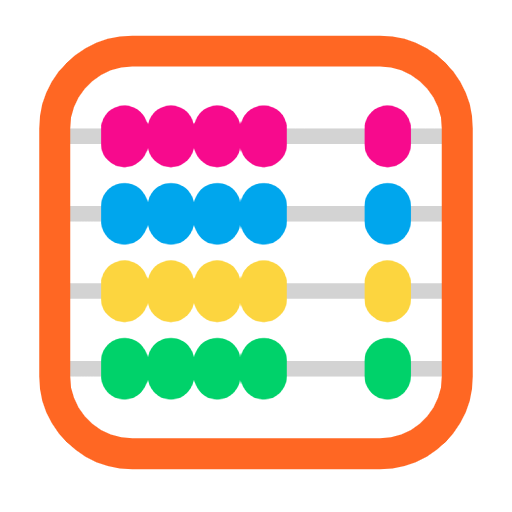
\includegraphics[width=30px]{images/abacus.png} & An invidual tallier can't decrypt anything, since it doesn't have the full tallier key.
        A group of talliers can decrypt ballots, but not see voters.
    \end{tabular}
\end{frame}

\begin{frame}{Other tricks}
    Aura has other properties, and can do other fun tricks. \\~\\

    \begin{table}
        \centering
        \begin{tabular}{>{\arraybackslash}m{40px} >{\arraybackslash}m{100px} >{\arraybackslash}m{220px}}
            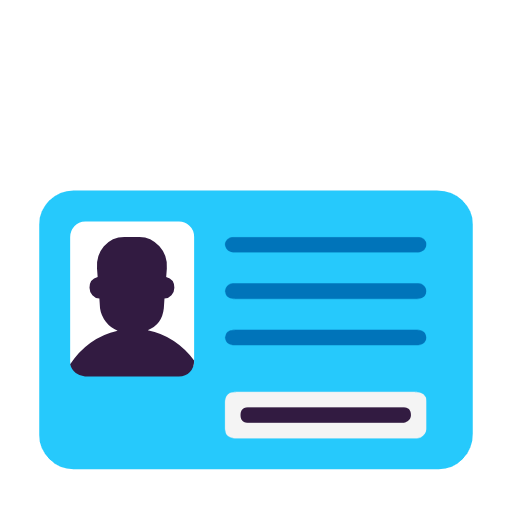
\includegraphics[width=30px]{images/id.png} & \textbf{No trusted setup} & All cryptographic plumbing can be constructed openly and verifiably. \\
            
\includegraphics[width=30px]{images/money.png} & \textbf{Coercion resistance} & The design can be modified to minimize risks of voter coercion or bribery, but with tradeoffs. \\
            
\includegraphics[width=30px]{images/key.png} & \textbf{Tallier key setup} & The tallier key is constructed and distributed in a safe and verifiable way. \\
            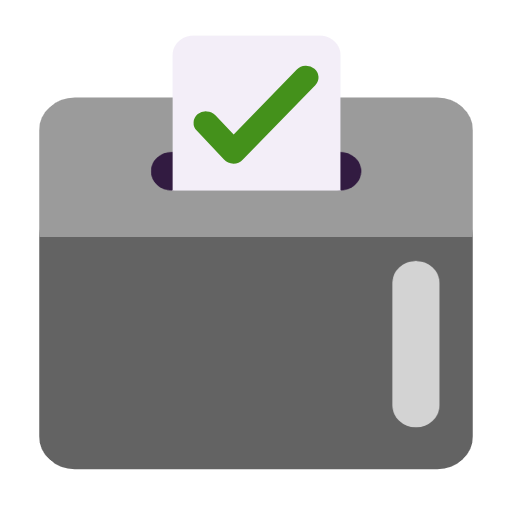
\includegraphics[width=30px]{images/ballot.png} & \textbf{Ballot selections} & Ballots can support a minimum and maximum number of allowed selections. \\
        \end{tabular}
    \end{table}
\end{frame}

\begin{frame}{Questions?}
	\Large
	\begin{center}
		\begin{tabular}{ll}
			\textbf{Preprint} & \url{ia.cr/2022/543} \\
			& \url{github.com/firoorg/aura-paper} \\
			\\
			\textbf{Slides} & \url{github.com/AaronFeickert/monkon2024} \\
			\\
			\textbf{Email} & \texttt{aaron@cypherstack.com}
		\end{tabular}
	\end{center}
\end{frame}

\end{document}
